
%(BEGIN_QUESTION)
% Copyright 2010, Tony R. Kuphaldt, released under the Creative Commons Attribution License (v 1.0)
% This means you may do almost anything with this work of mine, so long as you give me proper credit

Suppose a Fisher model 586 I/P converter is set up on a bench for a calibration test:

$$\includegraphics[width=15.5cm]{i00059x01.eps}$$

The ``As-Found'' calibration table for this converter tests as follows:

% No blank lines allowed between lines of an \halign structure!
% I use comments (%) instead, so that TeX doesn't choke.

$$\vbox{\offinterlineskip
\halign{\strut
\vrule \quad\hfil # \ \hfil & 
\vrule \quad\hfil # \ \hfil \vrule \cr
\noalign{\hrule}
%
% First row
Input current & Output pressure \cr
%
\noalign{\hrule}
%
% Another row
4.00 mA & 2.97 PSI \cr
%
\noalign{\hrule}
%
% Another row
8.00 mA & 5.98 PSI \cr
%
\noalign{\hrule}
%
% Another row
12.00 mA & 9.00 PSI \cr
%
\noalign{\hrule}
%
% Another row
16.00 mA & 11.37 PSI \cr
%
\noalign{\hrule}
%
% Another row
20.00 mA & 11.37 PSI \cr
%
\noalign{\hrule}
} % End of \halign 
}$$ % End of \vbox

Two fellow instrument technicians observing this test disagree as to the causes of the 75\% and 100\% errors.  One says this transducer has a {\it span} error and may be corrected by adjusting the span screw, while the other one says the problem cannot be corrected by any calibration (zero or span) adjustment.

What is your assessment of this instrument's problem?  Identify at least one realistic cause, and propose a remedy to correct the error.

\vfil

\underbar{file i00059}
\eject
%(END_QUESTION)





%(BEGIN_ANSWER)

This is a graded question -- no answers or hints given!

%(END_ANSWER)





%(BEGIN_NOTES)

A good problem-solving technique here is to sketch a graph of the input and output values for this instrument, to get a graphical representation of its behavior.  Sometimes this makes the problem easier to see than looking at a table of numbers:

$$\includegraphics[width=15.5cm]{i00059x02.eps}$$

From this graph we can clearly tell this I/P has a nonlinearity error!

\vskip 10pt

The most likely cause of the problem is insufficient air supply pressure.  Other possible causes include mis-alignment of the force-balance mechanism (causing it to ``jam'' in place at a certain amount of applied torque) and a partial leak in the nozzle tubing somewhere (causing nozzle backpressure to saturate at some maximum pressure below what it should be able to reach).

The second technician is correct: this is fundamentally a problem that cannot be corrected by any screw adjustment.  We know this is the case because the three calibration points of 4 mA, 8 mA, and 12 mA are very nearly right-on.  If it were a zero or a span problem, at least two of those three points would {\it also} be severely off-spec.  Also, no amount of zero or span error will cause the instrument to ``flat-line'' at the 75\% and 100\% points.  A zero adjustment would merely shift {\it all} the calibration points higher or lower.  A span adjustment would likewise affect all the calibration points to some extent, not cripple some while leaving others in nearly perfect condition! 

What we have here is extremely non-linear behavior.  Something is preventing the I/P's output pressure from exceeding 11.37 PSI.  


%INDEX% Calibration: table, I/P transducer
%INDEX% Relay, I/P transducer: Fisher model 546

%(END_NOTES)




